% Tex root = ../cheatsheet.tex
\section{Integralrechnung}
  \definition{4.1.1.1}{Integrale}
  Für $f:[a,b]\rightarrow\mathbb R^n$ ist\\
  $\int\limits_a^bf(t)dt:=\left(\int\limits_a^bf_1(t)dt,...,\int\limits_a^bf_n(t)dt\right)\in\mathbb
  R^n$
\subsection{Wegintegral}
  \definition{4.1.1.2}{Weg}
    Ein \textbf{Weg} ist ein stetiges $\gamma:[a,b]\rightarrow\mathbb R^n$. Man sagt
    $\gamma$ ist ein Weg \textbf{von $\gamma(a)$ nach $\gamma(b)$}. Wir betrachten
    nur Wege $\gamma$, die \textbf{stückweise $C^1$} sind, d.h. es gibt $k\geq1$
    und $a=t_0<t_1<\dots<t_k=b$ sodass $\gamma|_{(t_i-1,t_i)}$ für alle $1\leq i
    \leq k$ $C^1$ ist.\\
  \definition{4.1.1.3}{Wegintegral der Zweiten Art}
    Sei $\gamma:[a.b]\rightarrow\mathbb R^n$ ein Weg, $U\in\mathbb R^n$ mit
    Bild$(\gamma)\subseteq U$, und $f: U\rightarrow \mathbb R^n$ stetig. Dann
    ist das \textbf{Wegintegral von $f$ entlang $\gamma$} $$\int\limits_\gamma f(s)\cdot
    d\overrightarrow{s}:= \int\limits_a^b\left<f(\gamma(t)),\gamma'(t)\right>dt.$$
  \definition{4.1.4}{Orientierte Umparametrisierungen}
    Die OU eines Weges $\gamma:[a,b]\rightarrow\mathbb R^n$ ist ein Weg
    $\delta:[c,d]\rightarrow\mathbb R^n$ mit $\delta=\gamma\circ\varphi$, für ein
    $\varphi:[c,d]\rightarrow[a,b]$ welches stetig, diffbar auf $(c,d)$ und
    streng monoton wachsend ist mit $\varphi(c)=a, \varphi(d)=b$. (Insbesondere ist 
    $\varphi$ bijektiv.)\\
  \proposition{4.1.5}{Umparametriesierte Wegintegrale}
    Ist $\delta$ eine OU von $\gamma$, dann gilt $$\int\limits_\gamma f(s)\cdot
    d\overrightarrow{s}=\int\limits_\delta f(s)\cdot d\overrightarrow{s}$$
  \definition{4.1.8}{Konservative Vektorfelder}
    $U\in\mathbb R^n$, $f:U\rightarrow\mathbb R^m$ stetig. Falls für alle
    Punktpaare $v,w\in U$ und alle Wege $\gamma,\delta$ von $v$ nach $w$ gilt
    $$\int\limits_\gamma f(s)\cdot d\overrightarrow{s}=\int\limits_\delta f(s)\cdot
    d\overrightarrow{s}$$ dann heisst $f$ konservativ.\\
  \rmrk{4.1.9}{Geschlossene Wege}
    Ein Weg $\gamma:[a,b]\rightarrow\mathbb R^n$ mit $\gamma(a)=\gamma(b)$
    heisst geschlossen. Für solche wege kann man $\oint_\gamma$ schreiben.\\
  \proposition{}{Wegintegrale konservativer Felder über geschlossene Wege}
    $U\in\mathbb R^n$, $f:U\rightarrow\mathbb R^m$ konservativ $\iff
    \oint_\gamma f(s)\cdot d\overrightarrow{s}=0$ für alle geschlossenen Wege
    $\gamma:[a,b]\rightarrow U$.\\
  \definition{4.1.9.1}{Konvexe Mengen}
    $U\in\mathbb R^n$ heisst konvex, falls alle Strecken mit Endpunkten in $U$,
    selbst in $U$ enthalten sind.\\
  \definition{4.1.9.2}{Sternförmige Mengen}
    $U\in\mathbb R^n$ heisst sternförmig, falls es ein $x_0$ gibt, sodass für
    jedes $x\in U$ die Strecke mit Endpunkten $x, x_0$ in $U$ enthalten sind.\\
  \definition{4.1.9.3}{Wegzusammenhängende Mengen}
    $U\in\mathbb R^n$ heisst wegzusammenhängend, falls für alle $x,y\in U$ ein
    Weg von $x$ nach $y$ existiert.\\
  \rmrk{4.1.9.4}{Implikationen}
    Konvex $\implies$ Sternförmig $\implies$ Wegzusammenhängend.\\
  \proposition{4.1.9.5}{Sternförmige konservative felder}
    $U\in\mathbb R^n$ offen und \textbf{sternförmig}, $f\in C^1(U,\mathbb R^n)$ mit
    $\partial_if_j=\partial_jf_i\implies f$ konservativ.\\
  \proposition{4.1.10}{Potential}
    $U\in\mathbb R^n$ offen und $f:U\rightarrow\mathbb R^m$ konservativ. Dann
    gibt es ein $g\in C^1(U,\mathbb R)$ mit $f= \bigtriangledown g$. Ein solches
    $g$ heisst \textbf{Potential} von $f$. Falls $U$ wegzusammenhängend ist, dann ist das
    Potential bis auf addition einer Konstanten eindeutig.\\
  \proposition{4.1.13}{Jakobimatrix eines konservativen Feldes}
    $U\in\mathbb R^n$ offen, $f:U\rightarrow\mathbb R^m$ $C^1$. $f$ konservativ
    $\implies\partial_if_j=\partial_jf_i$ für $i,j\in\{1,...,n\}$ $\iff J_f(x)$
    symmetrisch für alle $x\in U$.\\
  \definition{4.1.20}{Rotation - Curl}
    $U\in\mathbb R^3$ offen, $f\in C^1(U,\mathbb R^3)$. Dann ist die Rotation
    von $f$ das $C^0$ Vektorfeld 
    $$ rot(f)=curl(f)=\begin{pmatrix}
      \partial_2f_3-\partial_3f_2\\
      \partial_3f_1-\partial_1f_3\\
      \partial_1f_2-\partial_2f_1
      \end{pmatrix} $$
  \rmrk{}{Übersicht konservativität}
    \begin{minipage}{\linewidth}
      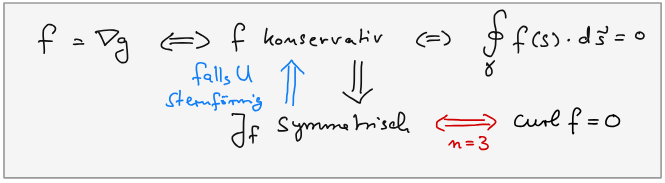
\includegraphics[width=\linewidth]{./media/uebersicht.png}
    \end{minipage}
\subsection{Das Riemannintegral in $\mathbb{R}^n$}
  Für $U\in\mathbb R^n$ kompakt und $f: U\rightarrow\mathbb R$ stetig kann man
  das Riemannintegral von $f$ über $U$ definieren, geschrieben
  $$\int\limits_Uf(x)dx\;\text{ oder }\int\limits_Uf(x_1,...,x_n)dx_1...dx_n$$
  Es ist gleich dem Rauminhalt, der in $R^{n+1}$ zwischen $U$ und dem Graphen
  von $f$ eingeschlossen wird, wobei anteile mit $f<0$ negativ sind.\\
  Eigenschaften des Riemannintegral in $\mathbb R^n$:\\
  \definition{4.2.0.1}{Kompatibilität}
    $n=1, U=[a,b]\implies\int\limits_Uf(x)dx=\int\limits_a^bf(x)dx$\\
  \definition{4.2.0.2}{Linearität}
    $\int\limits_Uaf(x)+bg(x)dx=a\int\limits_Uf(x)dx+b\int\limits_Ug(x)dx$\\
  \definition{4.2.0.3}{Inlkusion-Exklusion}
    $\int\limits_{U\cup V}f(x)dx=\int\limits_Uf(x)dx+\int\limits_Vf(x)dx-\int\limits_{U\cap V}f(x)dx$\\
  \definition{4.2.0.4}{Satz von Fubimi für 'Quader'}
    $U_1\in\mathbb R^{n_1}, U_2\in\mathbb R^{n_2}$ kompakt. Dann:
    $$\begin{array}{ll}
      \int\limits_{U\times
      V}f(x)dx&=\int\limits_{U_1}\left(\int\limits_{U_2}f(x_1,x_2)dx_2\right)dx_1\\
      &=\int\limits_{U_2}\left(\int\limits_{U_1}f(x_1,x_2)dx_1\right)dx_2
    \end{array}$$
  \definition{4.2.0.5}{Allgemeiner Satz von Fubimi}
    $U\subseteq\mathbb R^m=\mathbb R^{n_1}\times\mathbb R^{n_2}$\\
    $V=\{x_1\in\mathbb R^{n_1}\mid\exists x_2:(x_1,x_2)\in U\}\subseteq\mathbb
    R^{n_1}$\\
    $W(x_1)=\{x_2\in\mathbb R^{n_2}\mid(x_1,x_2)\in U\}\subseteq\mathbb
    R^{n_2}$\\
    Falls $g:V\rightarrow \mathbb R, g(x_1)=\int\limits_{W(x_1)}f(x_1,x_2)dx$ stetig
    ist, dann gilt $$\begin{array}{lcl}
      \int\limits_Uf(x)dx&=&\int\limits_Vg(x_1)dx_1\\
      &=&\int\limits_U\int\limits_{W(x_1)}f(x_1,x_2)dx_2dx_2
    \end{array}$$
  \definition{4.2.0.6}{Positivität}
    $f\leq g\implies\int\limits_Uf(x)dx\leq\int\limits_Ug(x)dx$\\
    $f\geq0,U\subseteq V\implies\int\limits_Uf(x)dx\leq\int\limits_Vf(x)dx$\\
  \definition{4.2.0.7}{Dreiecksungleichung}
    $\left|\int\limits_Uf(x)dx\right|\leq\int\limits_U\left|f(x)\right|dx$\\
  \definition{4.2.0.8}{Volumen}
    Das Volumen von $U$ ist definiert als $vol(U):=\int\limits_U1dx$. Der Satz von
    Fubimi kann zur berechnung des Volumens verwendet werden. zB Schnittfläche
    üver Höhe integrieren.\\
  \definition{4.2.3}{Parametrisierte und vernachlässigbare Mengen}
    \begin{enumerate}
      \item[(1)] Für $1\leq m\leq n$ ist eine \textbf{parametrisierte m-Menge} 
        in $\mathbb R^n$ eine stetige Funktion
        $$f:[a_1,b_1]\times\dots\times[a_m,b_m]\rightarrow\mathbb R^n$$ die
        $C^1$ auf $(a_1,b_1)\times\dots\times(a_m,b_m)$ ist.
      \item[(2)] $B\subseteq\mathbb R^n$ heisst \textbf{vernachlässigbar} falls
        $B\subseteq Bild(f_1)\cup\dots\cup Bild(f_n)$ für $m_i$-Mengen $f_i$ mit
        $m_i<n$.
    \end{enumerate}
  \proposition{4.2.5}{}
    Ist $U\subseteq\mathbb R^n$ kompakt und vernachlässigbar, dann
    $\int\limits_{U}f(x)dx=0$ für alle $f\in C^0(U,\mathbb R)$.\\
\subsection{Uneigentliche Integrale}
  Für $f:\mathbb R\rightarrow\mathbb R$ definiert man das uneigentliche Integral
  $$\int\limits_a^\infty
  f(x)dx:=\lim\limits_{b\rightarrow\infty}\int\limits_a^bf(x)dx$$
  \definition{4.3.0.1}{}
    Für $f:\mathbb R^2\rightarrow[0,\infty)$ stetig, ist $$\int\limits_{\mathbb
    R}f(x,y)dxdy=\lim\limits_{R\rightarrow\infty}\int\limits_{B_R(0)}f(x,y)dxdy$$
  \rmrk{4.3.0.2}{}
    $$\begin{array}{lcl}
      \int\limits_{\mathbb R^2}f(x,y)dxdy &=&
      \lim\limits_{S\rightarrow\infty}\int\limits_{[-S,S]^2}f(x,y)dxdy\\
      &=&\lim\limits_{S\rightarrow\infty}\int\limits_{-S}^S\int\limits_{-S}^Sf(x,y)dxdy
    \end{array}$$
    Falls $g(y)=\int\limits_{-\infty}^\infty f(x,y)dx$ für alle $y\in\mathbb
    R^2$ konvergiert und stetig ist, dann $$\int\limits_{\mathbb
    R^2}f(x,y)dxdy=\int\limits_{-\infty}^\infty\int\limits_{-\infty}^\infty
    f(x,y)dxdy$$
    \definition{4.3.1}{}
      $f:[a,\infty)\times[c,d]\rightarrow\mathbb R$ stetig, dann
      $$\int\limits_{[a,\infty)\times[c,d]}f(x,y)dxdy:=\lim\limits_{b\rightarrow\infty}
      \int\limits_{[a,b]\times[c,d]}f(x,y)dxdy$$
\subsection{Die Transformationsformel}
  \definition{4.4.0}{Substitutionsregel}
    $\int\limits_a^bf(g(x))g'(x)dx=\int\limits_{g(a)}^{g(b)}f(y)dy$\\
  \definition{4.4.2}{Transformationsformel}
    $$\int\limits_{\overline U}f(\varphi(x))|\det
    J_\varphi(x)|dx=\int\limits_{\overline V}f(y)dy$$
    falls:\begin{enumerate}
      \item[$*$] $\overline U$ kompakt, $\overline U=U\cup B$ mit $U$ offen, $B$
        vernachlässigbar
      \item[$*$] $\overline V$ kompakt, $\overline V=V\cup C$ mit $V$ offen, $C$
        vernachlässigbar
      \item[$*$] $f:\overline V\rightarrow\mathbb R$ stetig
      \item[$*$] $\varphi:\overline U\rightarrow\overline V$ stetig
      \item[$*$] $\varphi(U)=V, \varphi|_u$ injektiv und $C^1$
      \item[$*$] $|\det J_\varphi(x)|$ lässt sich stetig auf $\overline U$
        fortsetzen.
    \end{enumerate}
\subsection{Der Schwerpunkt}
  \definition{4.5.0}{Der Schwerpunkt}
    Der \textbf{Schwerpunkt} $\overline x\in\mathbb R^n$ einer kompakten Menge
    $U\in\mathbb R^n$ ist gegeben durch $\overline
    x_i=\frac{1}{vol(u)}\int\limits_Ux_idx$
\subsection{Satz von Green}
  \definition{4.6.1}{Einfache Geschlossene Kurve}
    Eine \textbf{einfach geschlossene Kurve} in $\mathbb R^n$ ist ein Weg
    $\gamma:[a,b]\rightarrow\mathbb R^n$, sodass für $s,t\in[a,b]$ mit $s<t$
    gilt: $$\gamma(s)=\gamma(t)\iff s=a\text{ und } t=b.$$
  \definition{4.6.3}{Satz von Green}
    $X\subseteq\mathbb R^2$ kompakt, mit Rand $\partial X$ gleich der disjunkten
    Vereinigung einfach geschlossener Kurven $\gamma_1,...,\gamma_k$. Ausserdem
    liege $X$ stets links von $\gamma_i$.
  \begin{minipage}{\linewidth}
    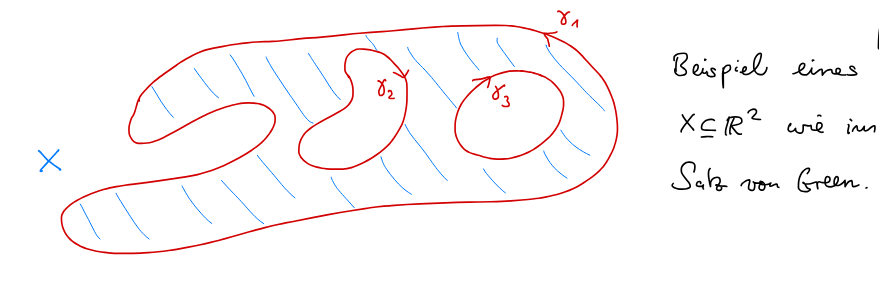
\includegraphics[width=\linewidth]{./media/satz_von_green.png}
  \end{minipage}
  $f:U\rightarrow\mathbb R^2$ ein $C^1$-Vektorfeld für ein offenes $U$ mit
  $X\subseteq U$. Dann: $$\int\limits_X\frac{\partial f_2}{\partial
  x}-\frac{\partial f_1}{\partial y}dxdy =
  \sum\limits_{i=1}^k\int\limits_{\gamma_i}f\cdot d\overrightarrow s.$$
  \vfil\null
